\documentclass[journal]{IEEEtran}
\usepackage[english]{babel}
\usepackage{%
  float,
  fullpage,
  indentfirst,
  thmtools,
  multicol,
  mathtools,
  cuted
}

% Define path where figures are stored
\newcommand{\figurepath}{../fig/bio}

\begin{document}

  \onecolumn
  \begin{multicols}{2}

    \begin{IEEEbiography}[{
\includegraphics[width=1in,height=1.25in,clip,keepaspectratio]{\figurepath/wiese.jpg}}]{Daniel Wiese}
      received his B.S. (2011) in mechanical engineering and aerospace science and engineering from the University of California, Davis.
      He completed his S.M. (2013) and Ph.D. (2016) at the Massachusetts Institute of Technology.
      His research interests include adaptive control, flight control, and control of hypersonic vehicles.
      His work has been in collaboration with Boeing and the US Air Force Research Lab at Wright-Patterson Air Force Base in Dayton, Ohio.
    \end{IEEEbiography}

    \begin{IEEEbiography}[{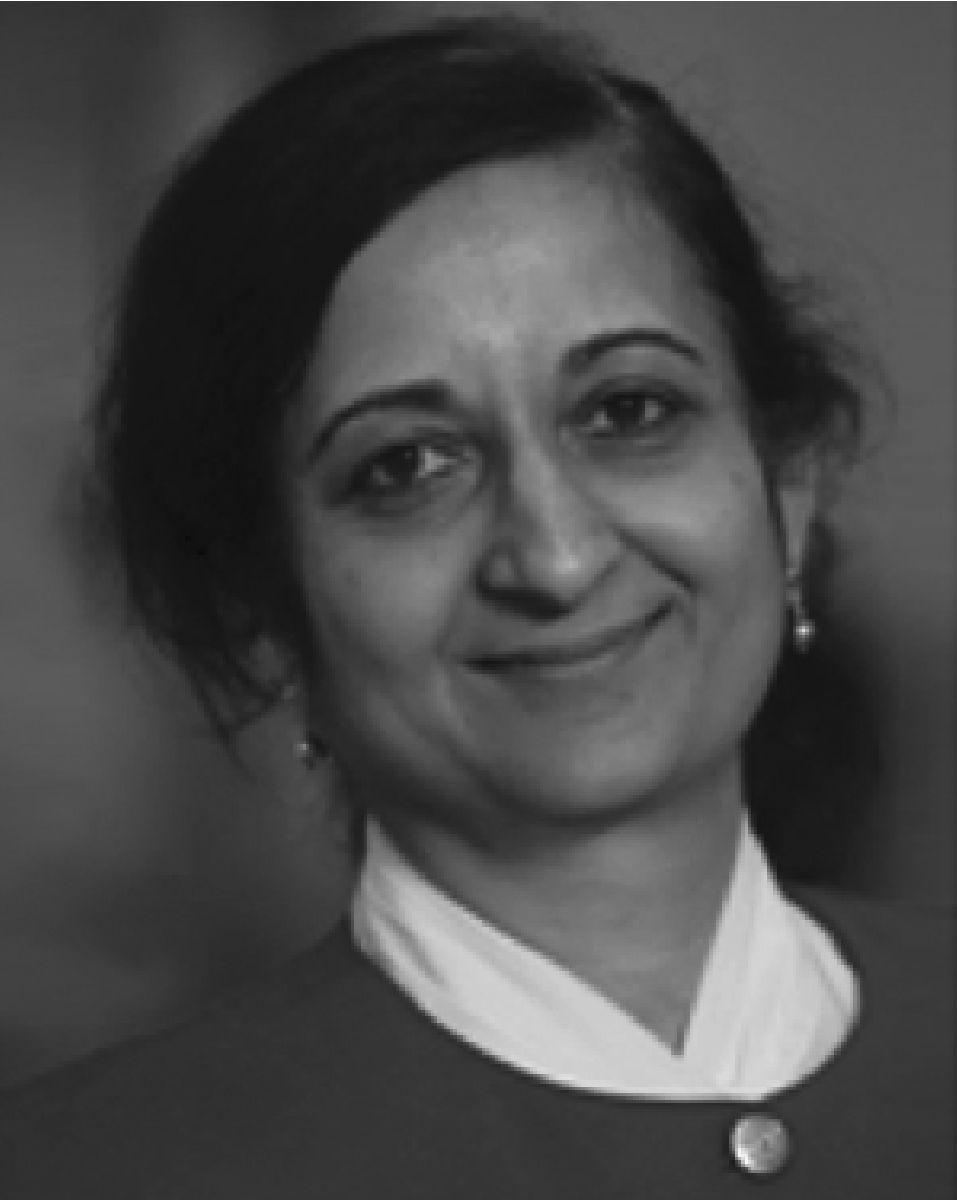
\includegraphics[width=1in,height=1.25in,clip,keepaspectratio]{\figurepath/annaswamy.png}}]{Anuradha Annaswamy}
      (S'82-M'85-SM'01-F'02) received the Ph.D. degree in electrical engineering from Yale University, New Have, CT, USA, in 1985.
      She has been a member of the faculty at Yale, Boston University, and MIT, where she is currently the Director of the Active-Adaptive Control Laboratory and a Senior Research Scientist in the Department of Mechanical Engineering.
      Her research interests pertain to adaptive control theory and applications to aerospace and automotive control, active control of noise in thermo-fluid systems, control of autonomous systems, decision and control in smart grids, and codesign of control and distributed embedded systems.
      She is the co-editor of the IEEE CSS report on ``Impact of Control Technology: Overview, Success Stories, and Research Challenges'', 2011, and the publication ``IEEE Vision for Smart Grid Control: 2030 and Beyond'', 2013.

      Dr.\ Annaswamy has received several awards including the George Axelby and Control Systems Magazine best paper awards from the IEEE Control Systems Society, the Presidential Young Investigator award from the National Science Foundation, the Hans Fisher Senior Fellowship from the Institute for Advanced Study at the Technische Universi{\"a}t M{\"u}nchen in 2008, and the Donald Groen Julius Prize for 2008 from the Institute of Mechanical Engineers.
      She is a member of AIAA.\@
    \end{IEEEbiography}

    \begin{IEEEbiography}[{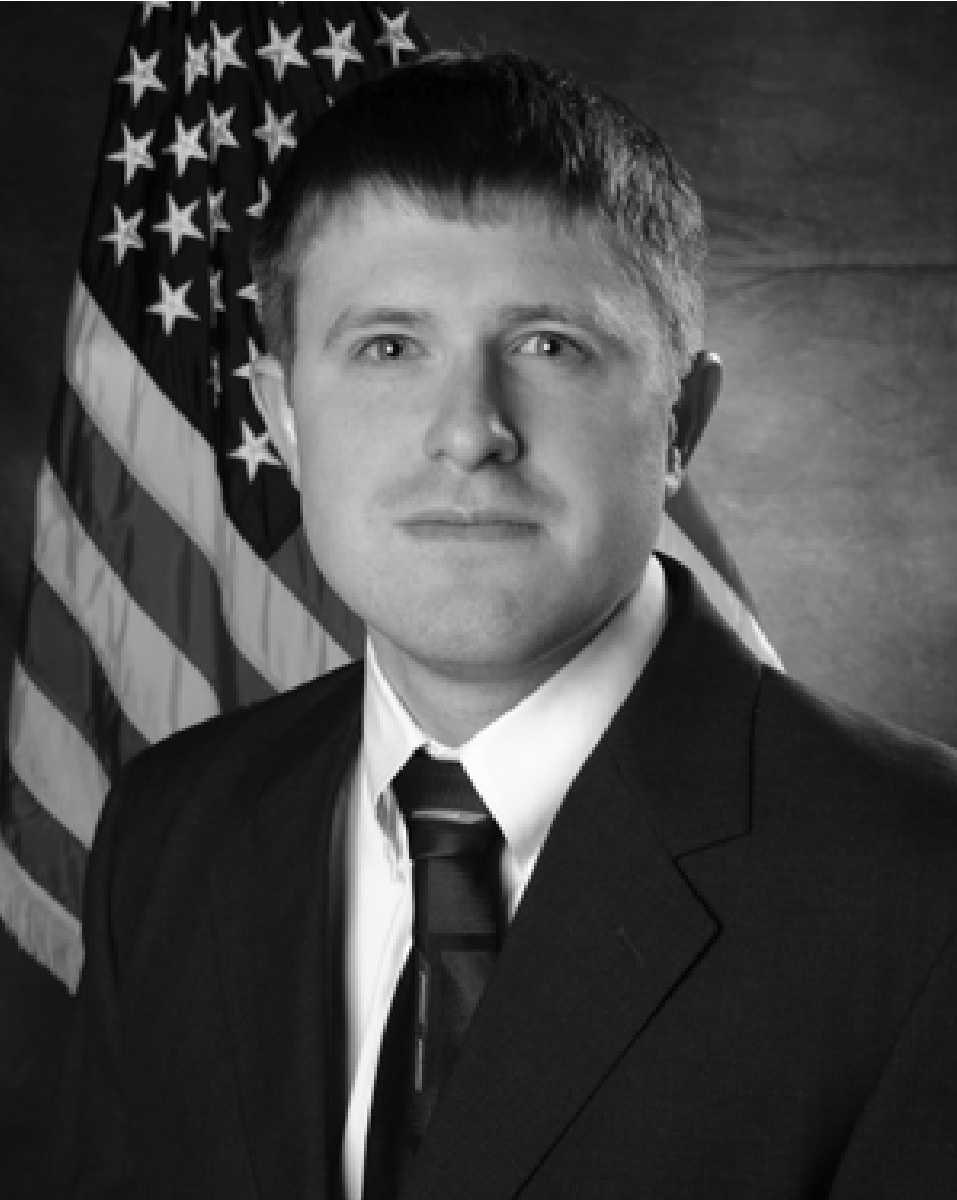
\includegraphics[width=1in,height=1.25in,clip,keepaspectratio]{\figurepath/muse.png}}]{Jonathan Muse}
      received the B.Sc.\ degree in aerospace engineering and mechanics from the University of Alabama, Tuscaloosa, AL, USA, in 2005, and the Ph.D. degree in aerospace engineering from the Georgia Institute of Technology, Atlanta, GA, USA, in 2010.
      He currently works at the Air Force Research Laboratory, Dayton, OH, USA, studying hypersonic vehicles and advanced methods in control theory while also serving as an Adjunct Professor with the Department of Electrical Engineering, Wright State University.
      He is also serving on several conference technical committees.
      He is on the Industrial Advisory Board for the University of Alabama's Aerospace Department, and has participated in multiple advisory roles in the aerospace industry.
    \end{IEEEbiography}

    \begin{IEEEbiography}[{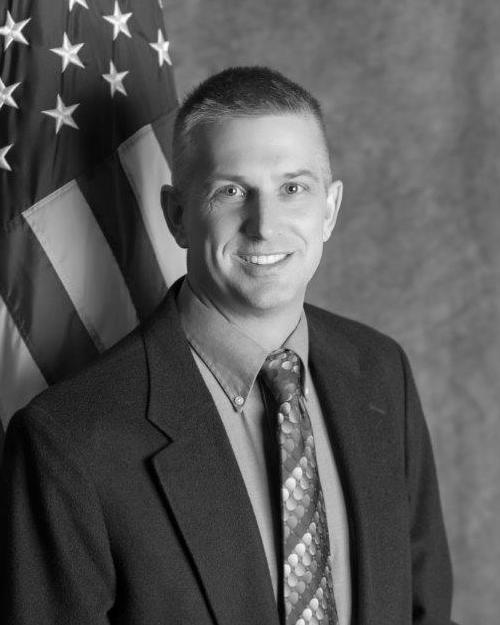
\includegraphics[width=1in,height=1.25in,clip,keepaspectratio]{\figurepath/bolender.jpg}}]{Michael Bolender}
      Michael A. Bolender received the Ph.D. degree from the University of Cincinnati in Aerospace Engineering in 2000.
      He is currently the Technical Area Lead for Hypersonic Vehicle Guidance and Flight Control in the Aerospace Systems Directorate within the U.S. Air Force Research Laboratory.
      His current research interests are the guidance and control of hypersonic vehicles, flight dynamics, and the application of control to complex aerospace systems.
      He is an Associate Fellow of AIAA.\@
    \end{IEEEbiography}

    \begin{IEEEbiography}[{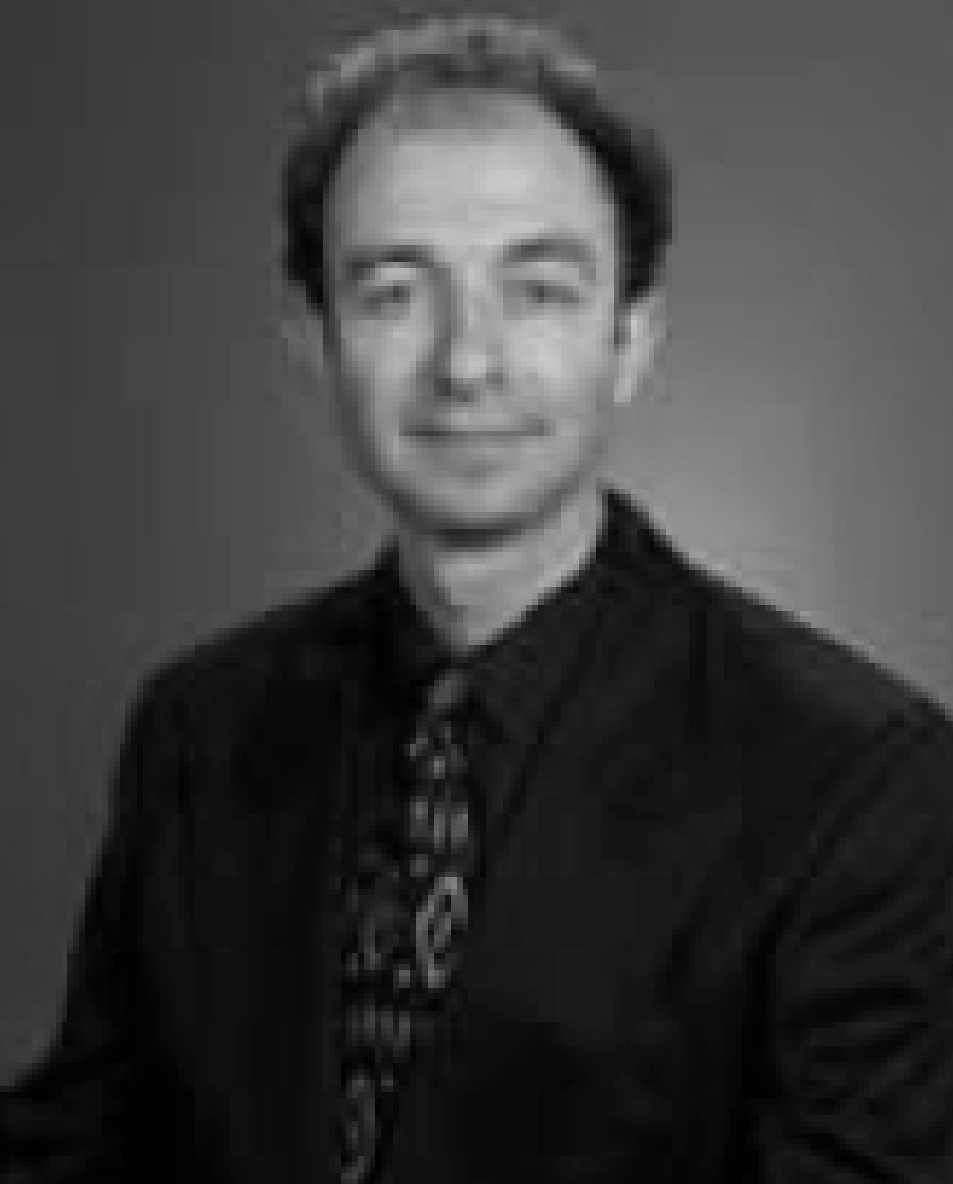
\includegraphics[width=1in,height=1.25in,clip,keepaspectratio]{\figurepath/lavretsky.png}}]{Eugene Lavretsky}
      received the M.S. degree in 1983 and the Ph.D. degree in 1999.
      He is a Boeing Senior Technical Fellow with Boeing Research and Technology, Huntington Beach, CA, USA.\@
      During his career at Boeing, he has developed flight control methods, system identification tools, and flight simulation technologies for transport aircraft, advanced unmanned aerial platforms, and weapon systems.
      Highlights include the MD-11 aircraft, NASA F/A-18 autonomous formation flight and high speed civil transport aircraft, JDAM guided munitions, X-45 and phantom ray autonomous aircraft, high altitude long endurance hydrogen-powered aircraft, and VULTURE solar-powered unmanned aerial vehicle.
      His research interests include robust and adaptive control and system identification and flight dynamics.
      He has written over 100 technical articles, and has taught graduate control courses at the California Long Beach State University, Long Beach, CA, USA, Claremont Graduate University, Claremont, CA, USA, California Institute of Technology, Pasadena, CA, USA, University of Missouri Science and Technology, Rolla, MO, USA, and the University of Southern California, Los Angeles, CA, USA.\@
      He is an Associate Fellow of AIAA.\@
      He is the recipient of the AIAA Mechanics and Control of Flight Award in 2009, the IEEE Control System Magazine Outstanding Paper Award in 2011, and the AACC Control Engineering Practice Award in 2012.
    \end{IEEEbiography}

  \end{multicols}

\end{document}
